\chapter{Testing}
This section provides information on the software and hardware tests of the NPSC. TIt starts by providing an overview of the model used to test the NPSC. It continues by providying all unit tests and system tests performed ont the NPSC. Lastly it explains the current, temperature and light experiments done on the Ring.
   
   
%%%%%%%%%%%%%%%%%%%%%%%%%%%%%%%%%%%%%%%%%%%%%%%%%%%%%%%%%%%%%%%%%%%%%%%%%%%%%%%%%%%%
% SECTION: Overview
%%%%%%%%%%%%%%%%%%%%%%%%%%%%%%%%%%%%%%%%%%%%%%%%%%%%%%%%%%%%%%%%%%%%%%%%%%%%%%%%%%%%
\section{Overview}
Debugging an embedded system is one of the worst thing in life, especially when there are logical errors in the program. In an embedded system like the NPSC which is made out of modules interacting with each other at different level of hierarchy, finding an error would be a difficult task as the error would have to be tracked down to the modules at lower levels. To reduce debugging time, it is essential that each module is indenpendently and thouroughly tested. To acheive this, the verification steps of the v-diagram of the NPSC shown in \cref{fig:v_diagram} are implemented.\\
The hardware modules and framework are tested by analysing the data transmitted between the STM and these hardware module and by running a set of unit tests on the framework code. The sub-systems of the NPSC are tested by running a set of software tests. Following the integration tests are the system test which consist of using the device to ensure that the system requirements have been met. The last verification steps consists of verifying that the device is an alarm-clock able to produce light of wavelength arround 460nm and able to fit in a $25*25*10 cm^3$ case. 
\begin{landscape} 
\begin{figure}[ht]
\centering
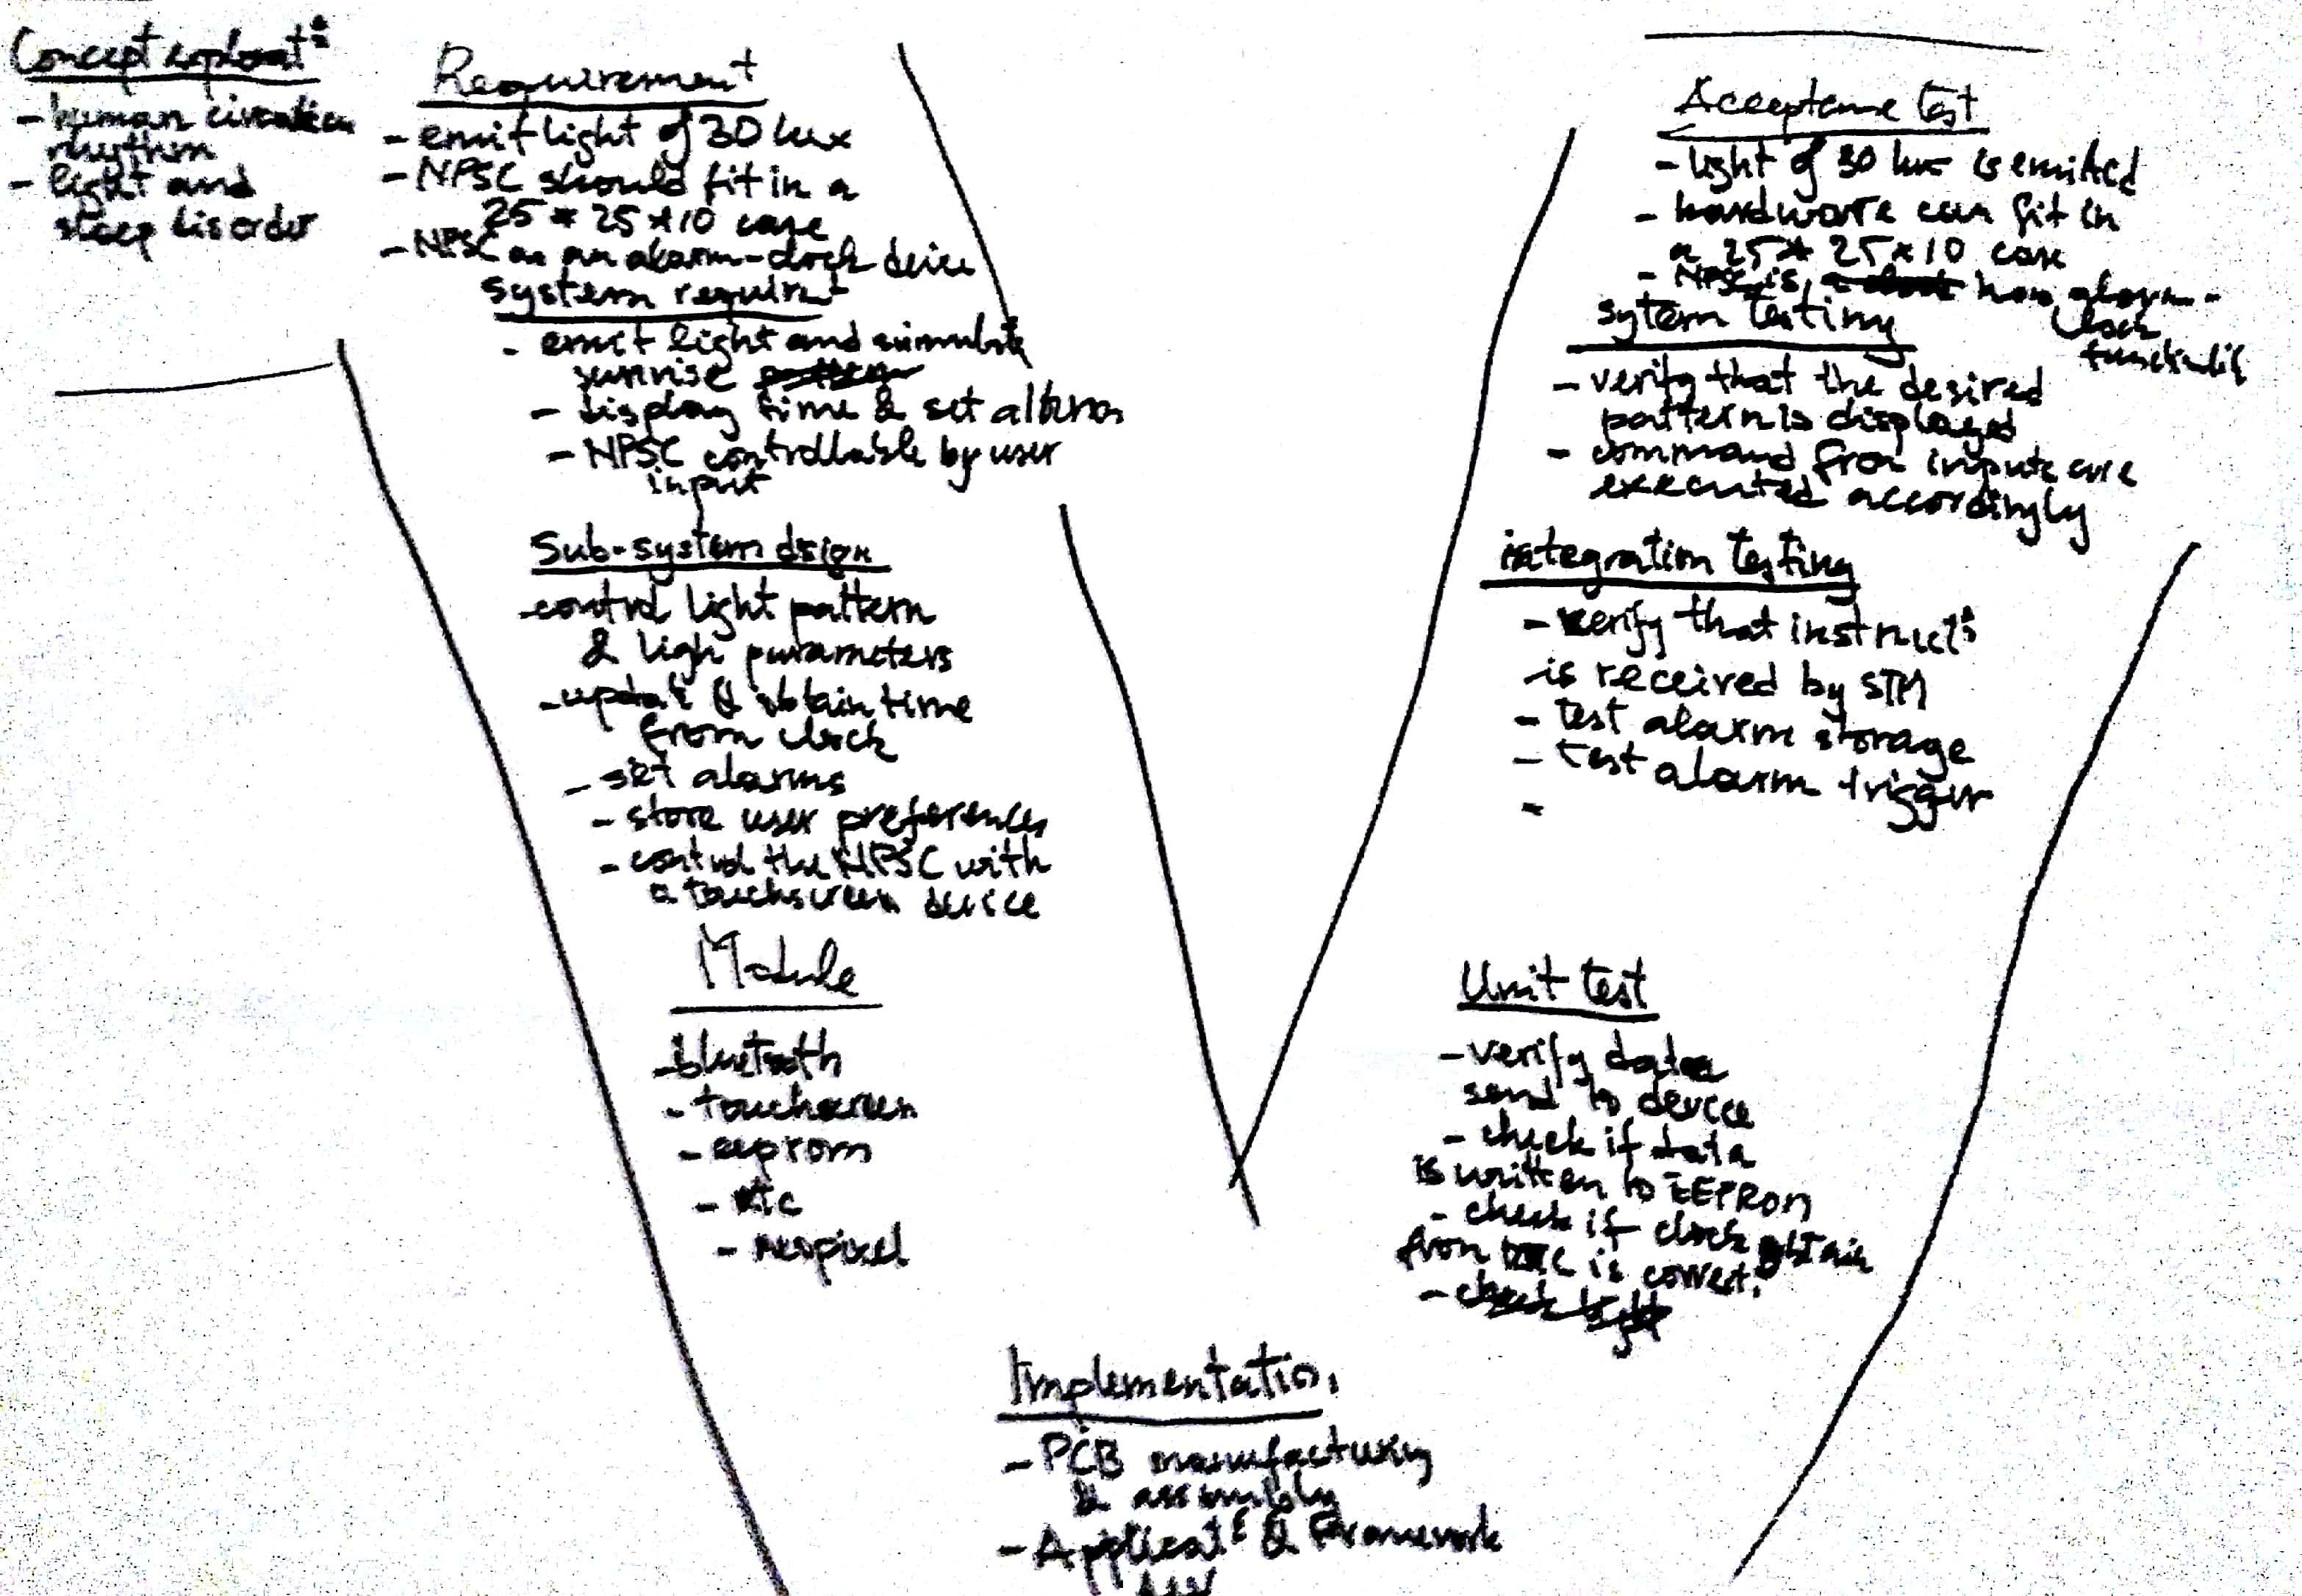
\includegraphics[scale=0.18]{v_diagram.jpg}
\caption{V-diagram of the project. On the left side, from top to bottom are the verifications steps starting from the system requirements down to the modules. At the bottom is the implementation of the ystem. On the right side, from the bottom to the top are the validations steps starting from the unit tests to the acceptance tests performed on the NPSC.}
\label{fig:v_diagram}
\end{figure}
\end{landscape}
%%%%%%%%%%%%%%%%%%%%%%%%%%%%%%%%%%%%%%%%%%%%%%%%%%%%%%%%%%%%%%%%%%%%%%%%%%%%%%%%%%%%
% SECTION: Hardware module
%%%%%%%%%%%%%%%%%%%%%%%%%%%%%%%%%%%%%%%%%%%%%%%%%%%%%%%%%%%%%%%%%%%%%%%%%%%%%%%%%%%%
\section{Hardware module tests}
The tests performed on the hardware are the basic harware tests mentioned in \ref{basic_hardware_test}.
To ensure that the hardware were sending and receiving the right information, the \textit{Salea logic analyser} was used to analyse the data transmitted between the STM and the hardware modules.\Cref{table:coms_test} describes the communication tests performed on each module.

\begin{table}[h!]
\centering
\caption{Commnication protocol tests performed on hardware modules.}
\label{table:coms_test}
\begin{tabular}{ccp{25em}}
\hline
\hline
\toprule
\textbf{Hardware} & \textbf{Protocol} & \textbf{Test description}\\
\hline
\hline
\toprule
DS1307 & I2C & \\ 
\midrule
25LC640 & SPI & \\ 
\midrule
HC-06 & UART & \\ 
\midrule
Nextion & UART & \\ 
\midrule
MAX & SPI & \\
\hline
\hline
\end{tabular}
\end{table}


   
%%%%%%%%%%%%%%%%%%%%%%%%%%%%%%%%%%%%%%%%%%%%%%%%%%%%%%%%%%%%%%%%%%%%%%%%%%%%%%%%%%%%
% SECTION: UnitTests
%%%%%%%%%%%%%%%%%%%%%%%%%%%%%%%%%%%%%%%%%%%%%%%%%%%%%%%%%%%%%%%%%%%%%%%%%%%%%%%%%%%%
\section{Unit tests}

Software unit tests could not be run on all hardware modules. It would have been impractical to set software unit tests on the Bluetooth module and the touchscreen as an application need to be developed using those module before fully interacting with them. The Utilities modules and the Framework of the hardware modules tested using unit testing are listed in \cref{table:unitTest} along side their unit tests.

\begin{table}[h!]
\centering
\caption{Unit tests performed on the Framework.}
\label{table:unitTest}
\begin{tabular}{ccp{18em}}
\hline
\hline
\textbf{Hardware} & \textbf{Unit test} & \textbf{Description}\\
\hline
\toprule
\multirow{6}{*}{internal RTC} & test\_clock\_date & Assert that the date saved is the same as the date loaded from the internal RTC\\
& test\_clock\_time & Assert that the time saved is the same as the time loaded from the internal RTC\\ 
& test\_clock\_alarm & Assert that the alarm saved is the same as the alarm loaded from the internal RTC\\
\midrule
\multirow{3}{*}{external RTC} & test\_rtc\_clock & Assert that the clock written to the external RTC is the same as the one loaded from the external RTC\\
\midrule
\multirow{6}{*}{queue} & test\_queue\_create & Assert that a queue of specific datatype has been created\\
& test\_queue\_enqueue & Assert that an element has been successfully added to the queue\\ 
& test\_queue\_dequeue & Assert that an element has been removed from the queue\\
\midrule
\multirow{9}{*}{eeprom} & test\_eeprom\_write\_read & Assert that the byte written to the eeprom is the same as the byte read at the written address.\\
& test\_eeprom\_write4B\_read4B & Assert that the a uint32\_t written to the eeprom is the same as the uint32\_t read at the written address.\\
& test\_eeprom\_writeNB\_readNB & Assert that the N bytes written to the eeprom are the same as the N bytes read at the written address.\\
\hline
\hline
\end{tabular}
\end{table}

%%%%%%%%%%%%%%%%%%%%%%%%%%%%%%%%%%%%%%%%%%%%%%%%%%%%%%%%%%%%%%%%%%%%%%%%%%%%%%%%%%%%
% SECTION: SystemTests
%%%%%%%%%%%%%%%%%%%%%%%%%%%%%%%%%%%%%%%%%%%%%%%%%%%%%%%%%%%%%%%%%%%%%%%%%%%%%%%%%%%%
\section{Integration tests}
\Cref{table:integrationTest} provides a description of all unit test performed on the hardware modules. 


\begin{table}[h!]
\centering
\caption{Description of the files at the Utilities level.}
\label{table:integrationTest}
\begin{tabular}{cp{30em}}
\hline
\hline
\toprule
\textbf{File Name} & \textbf{Description}\\
\bottomrule
\toprule
queue & Contains functions to create a queue of a certain data type, add and remove elements from the queue. \\
\midrule
utils & Contains functions, variables and type definitions used other software modules at different levels of the hierarchy.\\
\hline
\hline
\end{tabular}
\end{table}

%%%%%%%%%%%%%%%%%%%%%%%%%%%%%%%%%%%%%%%%%%%%%%%%%%%%%%%%%%%%%%%%%%%%%%%%%%%%%%%%%%%%
% SECTION: Ring
%%%%%%%%%%%%%%%%%%%%%%%%%%%%%%%%%%%%%%%%%%%%%%%%%%%%%%%%%%%%%%%%%%%%%%%%%%%%%%%%%%%%
\section{Neopixel Ring}
for each test:\\
** assumption\\
** how was each test performed in details, show pictures here
\subsection{Current test}
\subsection{Temperature test}
\subsection{Illuminance test}
